

\begin{frame}{Before we start...}
   \begin{block}{Ask Questions}
    \begin{itemize}
     \item Tell me if you do not understand
     \item Ask for further details
    \end{itemize}

   \end{block}

\end{frame}



\begin{frame}{Table of Contents}
   \begin{block}{About PETSc} \end{block}
   \begin{block}{First Steps} \end{block}
   \begin{block}{Application Integration} \end{block}
   \begin{block}{Profiling} \end{block}
   \begin{block}{PETSc and GPUs} \end{block}
\end{frame}


%%%%%% General PETSc information %%%%%%%%%%

%%% What is PETSc

%
% Stats, Who, Philosophy
%

%%%%%%%%%%%%%%%%%%%%%%%%%%%%

\section{About PETSc}
\begin{frame}{PETSc}
   \begin{center} \Large \textbf{About PETSc} \end{center}
\end{frame}


\input{slides/petsc-origins.tex}
\input{slides/Timeline}
\begin{frame}{PETSc}
\vspace*{-0.2cm}
\begin{center} {\bf Portable} Extensible Toolkit for Scientific Computing \end{center}
\vspace*{-0.2cm}

%\pause
\begin{block}{Architecture}
    \begin{itemize}  \vspace*{-0.2cm}
    \item tightly coupled (e.g. XT5, BG/P, Earth Simulator)
    \item loosely coupled such as network of workstations
    \item GPU clusters (many vector and sparse matrix kernels)
    \end{itemize}
\end{block} \vspace*{-0.2cm}


%\pause
\begin{block}{Software Environment}
  \begin{itemize}\vspace*{-0.2cm}
   \item Operating systems (Linux, Mac, Windows, BSD, proprietary Unix)
   \item Any compiler
   \item Usable from C, C++, Fortran 77/90, Python, and MATLAB
   \item Real/complex, single/double/quad precision, 32/64-bit int
  \end{itemize}
\end{block}\vspace*{-0.2cm}

%\pause
\begin{block}{System Size}
  \begin{itemize}\vspace*{-0.2cm}
   \item 500B unknowns, 75\% weak scalability on Jaguar (225k cores) \\
    and Jugene (295k cores)
   \item Same code runs performantly on a laptop
  \end{itemize}
\end{block}\vspace*{-0.2cm}

\begin{block}{Free to everyone (BSD-style license), open development}\end{block} \vspace*{-0.4cm}

\end{frame}


\begin{frame}{PETSc}

\begin{center}Portable {\bf Extensible} Toolkit for Scientific Computing \end{center}

%\pause
\begin{block}{Philosophy: Everything has a plugin architecture}
\begin{itemize}
  \item Vectors, Matrices, Coloring/ordering/partitioning algorithms
  \item Preconditioners, Krylov accelerators
  \item Nonlinear solvers, Time integrators
  \item Spatial discretizations/topology
\end{itemize}
\end{block}


%\pause
\begin{block}{Example}
  \begin{itemize}
   \item Vendor supplies matrix format and associated preconditioner, distributes
	compiled shared library.  
   \item Application user loads plugin at runtime, no source
	code in sight.
  \end{itemize}
\end{block}

\vspace{2cm}
\end{frame}


\begin{frame}{PETSc}

\begin{center} Portable Extensible {\bf Toolkit} for Scientific Computing \end{center}

%\pause
\begin{block}{Toolset}
  \begin{itemize}
   \item algorithms
   \item (parallel) debugging aids
   \item low-overhead profiling
  \end{itemize}
\end{block}

%\pause
\begin{block}{Composability}
 \begin{itemize}
  \item try new algorithms by choosing from product space
  \item composing existing algorithms (multilevel, domain decomposition, splitting)
 \end{itemize}
\end{block}
%}

%\pause
\begin{block}{Experimentation}
\begin{itemize}
  \item Impossible to pick the solver \emph{a priori}
  \item PETSc's response: expose an algebra of composition
  \item keep solvers decoupled from physics and discretization
\end{itemize}
\end{block}

\end{frame}

\begin{frame}{PETSc}
\vspace*{-0.2cm}
\begin{center}
 Portable Extensible Toolkit for {\bf Scientific Computing}
\end{center}
\vspace*{-0.2cm}

%\pause
  \begin{block}{Computational Scientists}
    \begin{itemize}\vspace*{-0.2cm}
    \item PyLith (CIG), Underworld (Monash), Magma Dynamics (LDEO, Columbia), PFLOTRAN (DOE), SHARP/UNIC (DOE)
    \end{itemize}
  \end{block}\vspace*{-0.2cm}

  
%\pause
\begin{block}{ Algorithm Developers (iterative methods and preconditioning)} \end{block}\vspace*{-0.4cm}


  %\pause
  \begin{block}{ Package Developers}
    \begin{itemize} \vspace*{-0.2cm}
    \item SLEPc, TAO, Deal.II, Libmesh, FEniCS, PETSc-FEM, MagPar, OOFEM, FreeCFD, OpenFVM
    \end{itemize}
  \end{block}\vspace*{-0.2cm}
%}

  %\pause
  \begin{block}{Funding}
    \begin{itemize} \vspace*{-0.2cm}    
      \item Department of Energy
      \begin{itemize}\item SciDAC, ASCR ISICLES, MICS Program, INL Reactor Program
      \end{itemize}
    \item National Science Foundation
      \begin{itemize}\item CIG, CISE, Multidisciplinary Challenge Program
      \end{itemize}
    \end{itemize}
  \end{block}\vspace*{-0.2cm}

  
  %\pause
  \begin{block}{Documentation and Support}
   \begin{itemize}\vspace*{-0.2cm}
    \item Hundreds of tutorial-style examples
    \item Hyperlinked manual, examples, and manual pages for all routines
    \item Support from \url{petsc-maint@mcs.anl.gov}
   \end{itemize}
  \end{block}

\end{frame}

\begin{frame}[fragile]

\frametitle{The Role of PETSc}

\vspace*{\fill}
\begin{minipage}{\linewidth}
\begin{quote}
\Large Developing parallel, nontrivial PDE solvers that deliver high performance is still difficult and requires
months (or even years) of concentrated effort.

\medskip

%\visible<2->{
PETSc is a toolkit that can ease these difficulties and reduce the development time, but it is not a black-box PDE
solver, \color{blue}{nor a silver bullet}.
\end{quote}
\qquad --- Barry Smith
%}
\end{minipage}


\end{frame}



%%%%%%%%%%%%%%%%%%%%%%%%%%%%

\section{First Steps}
\begin{frame}{PETSc}
   \begin{center} \Large \textbf{First Steps} \end{center}
\end{frame}


\begin{frame}[fragile]
\frametitle{PETSc}
 \begin{block}{Obtaining PETSc}
 \begin{itemize}
  \item http://mcs.anl.gov/petsc, download tarball
  \item Linux Package Managers
  \item Git: https://bitbucket.org/petsc/petsc
  \item Mercurial: https://bitbucket.org/petsc/petsc-hg
 \end{itemize}
 \end{block}

 \begin{block}{Installing PETSc}
 \begin{itemize}
  \item
 \begin{lstlisting}
  $> export PETSC_DIR=$PWD PETSC_ARCH=mpich-gcc-dbg
 \end{lstlisting}
  \item
 \begin{lstlisting}
  $> ./configure --with-shared-libraries
                 --with-blas-lapack-dir=/usr
                 --download-{mpich,ml,hypre}
\end{lstlisting}
  \item 
 \begin{lstlisting}
  $> make all test
 \end{lstlisting}
 \end{itemize}
 \end{block}

\end{frame}


\begin{frame}[fragile]
\frametitle{PETSc External Packages}

\begin{block}{Most packages can be automatically}
  \begin{itemize}  \vspace*{-0.2cm}
    \item Downloaded
    \item Configured and Built (in \lstinline|$PETSC_DIR/externalpackages|)
    \item Installed with PETSc
  \end{itemize}
\end{block} \vspace*{-0.2cm}
  
  %\pause
\begin{block}{Works for (list incomplete)}
  \begin{itemize}  \vspace*{-0.2cm}
    \item petsc4py
    \item PETSc documentation utilities (Sowing, lgrind, c2html)
    \item BLAS, LAPACK, BLACS, ScaLAPACK, PLAPACK
    \item MPICH, MPE, OpenMPI
    \item ParMetis, Chaco, Jostle, Party, Scotch, Zoltan
    \item MUMPS, Spooles, SuperLU, SuperLU\_Dist, UMFPack, pARMS
    \item PaStiX, BLOPEX, FFTW, SPRNG
    \item Prometheus, HYPRE, ML, SPAI
    \item Sundials
    \item Triangle, TetGen, FIAT, FFC, Generator
    \item HDF5, Boost
  \end{itemize}
\end{block}

\end{frame}




\begin{frame}[fragile]
\frametitle{PETSc Pyramid}
 \begin{block}{PETSc Structure} \vspace{0.3cm}
   \includegraphics[width=1.0\textwidth]{PETScPyramid.jpg}
 \end{block}

\end{frame}

\begin{frame}[fragile]
\frametitle{Flow Control for a PETSc Application}

\begin{center}
\includegraphics[width=4.0in]{figures/FlowControl}
\end{center}
\end{frame}



\begin{frame}[fragile]
\frametitle{PETSc Objects}
\begin{block}{Sample Code}
  \begin{lstlisting}
    Mat A;
    PetscInt m,n,M,N;
    MatCreate(comm,&A);
    MatSetSizes(A,m,n,M,N);      /* or PETSC_DECIDE */ 
    MatSetOptionsPrefix(A,"foo_");
    MatSetFromOptions(A);
    /* Use A */
    MatView(A,PETSC_VIEWER_DRAW_WORLD);
    MatDestroy(A);
  \end{lstlisting}
  \end{block}
  
  \begin{block}{Remarks}
  \begin{itemize}
  \item \lstinline|Mat| is an opaque object (pointer to incomplete type)
    \begin{itemize}
     \item Assignment, comparison, etc, are cheap
    \end{itemize}
  \item What's up with this ``Options'' stuff?
    \begin{itemize}
    \item We will discuss this later...
    \end{itemize}
  \end{itemize}
  
\end{block}
\end{frame}

\begin{frame}{Basic PetscObject Usage}

\begin{block}{Every object in PETSc supports a basic interface}
\vspace{0.3cm}
\begin{tabular}{|r|l|}
\hline
Function & Operation \\
\hline
\texttt{Create()}               & create the object \\
\texttt{Get/SetName()}          & name the object \\
\texttt{Get/SetType()}          & set the implementation type \\
\texttt{Get/SetOptionsPrefix()} & set the prefix for all options \\
\texttt{SetFromOptions()}       & customize object from command line \\
\texttt{SetUp()}                & perform other initialization \\
\texttt{View()}                 & view the object \\
\texttt{Destroy()}              & cleanup object allocation \\
\hline
\end{tabular}

\end{block}

\begin{block}{Also, all objects support the \lstinline|-help| option.}\end{block}

\end{frame}


\begin{frame}[fragile]{PETSc Options}
\begin{block}{Ways to set options}
  \begin{itemize}
  \item Command line
  \item Filename in the third argument of \lstinline|PetscInitialize()|
  \item \lstinline|~/.petscrc|
  \item \lstinline|$PWD/.petscrc|
  \item \lstinline|$PWD/petscrc|
  \item \lstinline|PetscOptionsInsertFile()|
  \item \lstinline|PetscOptionsInsertString()|
  \item \lstinline|PETSC_OPTIONS| environment variable
  \item command line option \lstinline|-options_file [file]|
  \end{itemize}
\end{block}
\end{frame}


\begin{frame}[fragile]{PETSc Options}

\begin{block}{Example of Command Line Control}
  %\lstinline|$> cd $PETSC_DIR/src/snes/examples/tutorials && make ex5}| \\
  \begin{itemize}
  \item \lstinline|$> ./ex5 -da_grid_x 10 -da_grid_y 10 -par 6.7| \\
      \lstinline|       -snes_monitor -{ksp,snes}_converged_reason| \\
      \lstinline|       -snes_view|
  \item \lstinline|$> ./ex5 -da_grid_x 10 -da_grid_y 10 -par 6.7| \\
      \lstinline|       -snes_monitor -{ksp,snes}_converged_reason| \\
      \lstinline|       -snes_view -mat_view_draw -draw_pause 0.5|
  \item \lstinline|$> ./ex5 -da_grid_x 10 -da_grid_y 10 -par 6.7| \\
      \lstinline|       -snes_monitor -{ksp,snes}_converged_reason| \\
      \lstinline|       -snes_view -mat_view_draw -draw_pause 0.5| \\
      \lstinline|       -pc_type lu -pc_factor_mat_ordering_type natural|
  \item Use \lstinline|-help| to find other ordering types
\end{itemize}
\end{block}
\end{frame}


%%%%%%%%%%%%%%%%%%%%%%%%%%%%

\section{Application Integration}
\begin{frame}{PETSc}
   \begin{center} \Large \textbf{Application Integration} \end{center}
\end{frame}

\begin{frame}{Application Integration}

\begin{block}{Be willing to experiment with algorithms}
  \begin{itemize}
    \item No optimality without interplay between physics and algorithmics
  \end{itemize}
\end{block}

\begin{block}{Adopt flexible, extensible programming}
  \begin{itemize}
    \item Algorithms and data structures not hardwired
  \end{itemize}
\end{block}

\begin{block}{Be willing to play with the real code}
  \begin{itemize}
    \item Toy models have limited usefulness
    \item But make test cases that run quickly
  \end{itemize}
\end{block}

\begin{block}{If possible, profile before integration}
  \begin{itemize}
    \item Automatic in PETSc
  \end{itemize}
\end{block}

\end{frame}

\begin{frame}[fragile]{Incorporating PETSc into Existing Codes}
  \begin{block}{PETSc does not seize \lstinline|main()|, does not control output}   \end{block} \vspace*{-0.4cm}
  %\pause
  \begin{block}{Propogates errors from underlying packages, flexible}   \end{block} \vspace*{-0.4cm}
  %\pause
  \begin{block}{Nothing special about \lstinline|MPI_COMM_WORLD|}   \end{block} \vspace*{-0.4cm}
  %\pause
  \begin{block}{Can wrap existing data structures/algorithms}
    \begin{itemize} \vspace*{-0.2cm}
    \item \lstinline|MatShell|, \lstinline|PCShell|, full implementations
    \item \lstinline|VecCreateMPIWithArray()|
    \item \lstinline|MatCreateSeqAIJWithArrays()|
    \item Use an existing semi-implicit solver as a preconditioner
    \item Usually worthwhile to use native PETSc data structures \\
      unless you have a good reason not to
    \end{itemize}
  \end{block} \vspace*{-0.4cm}
  %\pause
  \begin{block}{Uniform interfaces across languages}
    \begin{itemize} \vspace*{-0.2cm}
    \item C, C++, Fortran 77/90, Python, MATLAB
    \end{itemize}
  \end{block} \vspace*{-0.4cm}
  %\pause
  \begin{block}{Do not have to use high level interfaces (e.g.~SNES, TS, DM)}
    \begin{itemize} \vspace*{-0.2cm}
    \item but PETSc can offer more if you do, like MFFD and SNES Test
    \end{itemize}
  \end{block}
\end{frame}

\input{slides/Stages.tex}
\begin{frame}[fragile]{Initialization}

\begin{block}{Call \lstinline|PetscInitialize()|}
  \begin{itemize}
    \item Setup static data and services
    \item Setup MPI if it is not already
    \item Can set \lstinline|PETSC_COMM_WORLD| to use your communicator \\
      (can always use subcommunicators for each object)
  \end{itemize}
\end{block}

\begin{block}{Call \lstinline|PetscFinalize()|}
  \begin{itemize}
    \item Calculates logging summary
    \item Can check for leaks/unused options
    \item Shutdown and release resources
  \end{itemize}
\end{block}

\begin{block}{Can only initialize PETSc once}
\end{block}

\end{frame}


\begin{frame}[fragile]{PETSc Application Integration}

\begin{block}{Sparse Matrices}
\begin{itemize}
  \item \textbf{The} important data type when solving PDEs
  \item Two main phases: 
    \begin{itemize}
     \item Filling with entries (assembly)
     \item Application of its action (e.g.~SpMV)
    \end{itemize}
\end{itemize}
\end{block}
\begin{center}
%\includegraphics[width=2in]{figures/Mat/serialSparseMatrix_bcsstk32}
\includegraphics[width=.5\textwidth]{figures/EllipRCMSquare}
\end{center}
\end{frame}



\begin{frame}[fragile]{Matrix Memory Preallocation}
 \begin{block}{PETSc sparse matrices are dynamic data structures}
  \begin{itemize} \vspace*{-0.2cm}
    \item can add additional nonzeros freely
  \end{itemize}
 \end{block}  \vspace*{-0.2cm}

 %\pause
 \begin{block}{Dynamically adding many nonzeros}
  \begin{itemize} \vspace*{-0.2cm}
    \item requires additional memory allocations
    \item requires copies
    \item can kill performance
  \end{itemize}
 \end{block} \vspace*{-0.2cm}

 %\pause
 \begin{block}{Memory preallocation provides}
  \begin{itemize} \vspace*{-0.2cm}
    \item the freedom of dynamic data structures
    \item good performance
  \end{itemize}
 \end{block} \vspace*{-0.2cm}

 %\pause
 \begin{block}{Easiest solution is to replicate the assembly code}
  \begin{itemize} \vspace*{-0.2cm}
    \item Remove computation, but preserve the indexing code
    \item Store set of columns for each row
  \end{itemize}
 \end{block} \vspace*{-0.2cm}

 %\pause
 \begin{block}{Call preallocation routines for all datatypes}
  \begin{itemize} \vspace*{-0.2cm}
    \item \lstinline|MatSeqAIJSetPreallocation()|
    \item \lstinline|MatMPIBAIJSetPreallocation()|
    \item Only the relevant data will be used
  \end{itemize}
\end{block}
\end{frame}




\begin{frame}[fragile]{PETSc Application Integration}

\begin{block}{Sequential Sparse Matrices}
\lstinline|MatSeqAIJSetPreallocation(Mat A, int nz, int nnz[])|
\hbox{\qquad
\vbox{
\begin{itemize}
  \item[nz:] expected number of nonzeros in any row
  \item[nnz(i):] expected number of nonzeros in row i
\end{itemize}
}
}
\end{block}
\begin{center}
%\includegraphics[width=2in]{figures/Mat/serialSparseMatrix_bcsstk32}
\includegraphics[width=.5\textwidth]{figures/EllipRCMSquare}
\end{center}
\end{frame}

\begin{frame}[fragile]{PETSc Application Integration}

\begin{block}{Parallel Sparse Matrix}
\begin{itemize}
  \item Each process locally owns a submatrix of contiguous global rows
  \item Each submatrix consists of diagonal and off-diagonal parts
\end{itemize}

\begin{center}
\includegraphics[width=3.in]{figures/Mat/parallelSparseMatrix}
\end{center}

\begin{itemize}
  \item \lstinline|MatGetOwnershipRange(Mat A,int *start,int *end)|
  \begin{itemize}
    \item \lstinline|start|: first locally owned row of global matrix
    \item \lstinline|end-1|: last locally owned row of global matrix
  \end{itemize}
\end{itemize}
\end{block}
\end{frame}


\begin{frame}[fragile]{PETSc Application Integration}

\begin{center}
\includegraphics[width=3.in]{figures/Mat/parallelSparseMatrix}
\end{center}

\begin{center}
\begin{tabular}{cc}
\begin{tabular}{c}
\begin{tabular}{|ccc|cc|}
\hline
\multicolumn{3}{|c|}{Proc 2} & \multicolumn{2}{c|}{Proc 3} \\
\hline
25 & 26 & 27 & 28 & 29 \\
20 & 21 & 22 & 23 & 24 \\
15 & 16 & 17 & 18 & 19 \\
\hline
10 & 11 & 12 & 13 & 14 \\
 5 &  6 &  7 &  8 &  9 \\
 0 &  1 &  2 &  3 &  4 \\
\hline
\multicolumn{3}{|c|}{Proc 0} & \multicolumn{2}{c|}{Proc 1} \\
\hline
\end{tabular} \\
Natural numbering
\end{tabular}
& 
\begin{tabular}{c}
\begin{tabular}{|ccc|cc|}
\hline
\multicolumn{3}{|c|}{Proc 2} & \multicolumn{2}{c|}{Proc 3} \\
\hline
21 & 22 & 23 & 28 & 29 \\
18 & 19 & 20 & 26 & 27 \\
15 & 16 & 17 & 24 & 25 \\
\hline
 6 &  7 &  8 & 13 & 14 \\
 3 &  4 &  5 & 11 & 12 \\
 0 &  1 &  2 &  9 & 10 \\
\hline
\multicolumn{3}{|c|}{Proc 0} & \multicolumn{2}{c|}{Proc 1} \\
\hline
\end{tabular}\\
PETSc numbering
\end{tabular}
\end{tabular}
\end{center}

\end{frame}








\begin{frame}[fragile]{PETSc Application Integration}

\begin{block}{Parallel Sparse Matrix}
\vspace{0.5cm}
\hbox{ \quad \vbox{
\begin{lstlisting}
 MatMPIAIJSetPreallocation(Mat A, int dnz, int dnnz[],
                                  int onz, int onnz[]
\end{lstlisting}

\begin{itemize}
  \item[dnz:] expected number of nonzeros in any row in the diagonal block
  \item[dnnz(i):] expected number of nonzeros in row i in the diagonal block
  \item[onz:] expected number of nonzeros in any row in the offdiagonal portion
  \item[onnz(i):] expected number of nonzeros in row i in the offdiagonal portion
\end{itemize}
}}
\end{block}
\end{frame}

\begin{frame}[fragile]{PETSc Application Integration}

\begin{block}{Verifying Preallocation}
\begin{itemize}
  \item Use runtime options 
    \begin{itemize}
      \item \lstinline|-mat_new_nonzero_location_err| 
      \item \lstinline|-mat_new_nonzero_allocation_err|
    \end{itemize}
    
  \item Use runtime option
    \begin{itemize} \item \lstinline|-info| \end{itemize}
  \item Output: \\
\end{itemize}

\end{block}
\begin{lstlisting}[basicstyle=\scriptsize]
[proc #] Matrix size: %d X %d; storage space: %d unneeded, %d used
[proc #] Number of mallocs during MatSetValues( )  is %d
\end{lstlisting}

\begin{center}
\includegraphics[width=4.in]{figures/logInfoOutput}
\end{center}
\end{frame}

\begin{frame}[fragile]{Block and Symmetric Formats}
  \begin{block}{BAIJ}
    \begin{itemize}
    \item Like AIJ, but uses static block size
    \item Preallocation is like AIJ, but just one index per block
    \end{itemize}
  \end{block}
  
  %\pause
  \begin{block}{SBAIJ}
    \begin{itemize}
    \item Only stores upper triangular part
    \item Preallocation needs number of nonzeros in upper triangular \\
      parts of on- and off-diagonal blocks
    \end{itemize}
  \end{block}
    
  %\pause
  \begin{block}{MatSetValuesBlocked()}
    \begin{itemize}
    \item Better performance with blocked formats
    \item Also works with scalar formats, if \lstinline|MatSetBlockSize()| was called
    \item Variants \lstinline|MatSetValuesBlockedLocal()|, \lstinline|MatSetValuesBlockedStencil()|
    \item Change matrix format at runtime, don't need to touch assembly code
    \end{itemize}
  \end{block}
\end{frame}


%%%%%%%%%%%%%%%%%%%%%%%%%%%%

\section{Matrices in PETSc}
\begin{frame}{Matrices}
  \begin{definition}[Matrix]
    A \alert{matrix} is a linear transformation between finite dimensional vector spaces.
  \end{definition}
  \begin{definition}[Forming a matrix]
    \alert{Forming} or \alert{assembling} a matrix means defining it's action in terms of entries (usually stored in a sparse format).
  \end{definition}
\end{frame}

\input{slides/MatricesImportant.tex}
\begin{frame}{Matrices}

\begin{center}
 \em What can we do with a matrix that doesn't have entries?
\end{center}

 %\pause

  \begin{block}{Krylov solvers for $A x = b$}
    \begin{itemize}
    \item Krylov subspace: $\{b, Ab, A^2b, A^3b, \dotsc\}$
    \item Convergence rate depends on the spectral properties of the matrix
      %\begin{itemize}
      %\item Existance of small polynomials $p_n(A) < \epsilon$ where $p_n(0) = 1$.
      %\item condition number $\kappa(A) = \Vert A \Vert \Vert A^{-1} \Vert = \sigma_{\text{max}}/\sigma_{\text{min}}$
      %\item distribution of singular values, spectrum $\Lambda$, pseudospectrum $\Lambda_\epsilon$
%      \item $\epsilon$-pseudospectrum $\Lambda_\epsilon$, spectrum of $A + E$ where $\norm{E} < \epsilon$
      %\end{itemize}
    \item For any popular Krylov method $\mathcal{K}$, there is a matrix
      of size $m$, such that $\mathcal{K}$ outperforms all other methods
      by a factor at least $\mathcal{O}(\sqrt{m})$~[Nachtigal et. al., 1992]%\cite{nachtigal1992fnm}
    \end{itemize}
  \end{block}
  
%\pause

  \begin{block}{Typically...}
    \begin{itemize}
    \item The action $y \gets A x$ can be computed in $\mathcal{O}(m)$
    \item Aside from matrix multiply, the $n^{\text{th}}$ iteration requires at most $\mathcal{O}(mn)$
    \end{itemize}
  \end{block}
\end{frame}

\input{slides/GMRES.tex}
\begin{frame}[fragile]{PETSc Solvers}

\begin{block}{Linear Solvers - Krylov Methods}
 \begin{itemize}
  \item Using PETSc linear algebra, just add:
  \begin{lstlisting}[basicstyle=\footnotesize\ttfamily]
KSPSetOperators(KSP ksp, Mat A, Mat M, MatStructure flag)
KSPSolve(KSP ksp, Vec b, Vec x)
  \end{lstlisting}

  \item Can access subobjects
  \begin{lstlisting}[basicstyle=\footnotesize\ttfamily]
KSPGetPC(KSP ksp, PC *pc)
  \end{lstlisting}

  \item Preconditioners must obey PETSc interface
  \begin{itemize}
    \item Basically just the KSP interface
  \end{itemize}

  \item Can change solver dynamically from the command line, \lstinline|-ksp_type|
\end{itemize}
\end{block}

\end{frame}

\begin{frame}{Newton iteration: workhorse of SNES}
  \begin{flushright}
    \includegraphics[width=0.25\textwidth]{figures/Newton}
  \end{flushright}
  \vspace*{-4cm}
  \begin{block}{Standard form of a nonlinear system}
    \[ F(u) = 0 \]
  \end{block}
  
  \begin{block}{Iteration}
    \begin{align*}
      \text{Solve:} & \qquad J(u) w = -F(u) \\
      \text{Update:} & \qquad u^+ \gets u + w
    \end{align*}
    \begin{itemize}
    \item Quadratically convergent near a root: $|u^{n+1}-u^*| \in \mathcal{O} \Big(|u^n-u^*|^2\Big)$
    \item Picard is the same operation with a different $J(u)$
    \end{itemize}
  \end{block}
  
%\begin{block}{Nonlinear Poisson}
%    \begin{align*}
%      F(u)=0 \quad &\sim\quad -\div\big[ (1+u^2) \grad u \big] - f = 0 \\
%      J(u)w \quad &\sim\quad  -\div\big[(1+u^2)\grad w + 2uw\grad u \Big]
%    \end{align*}
%\end{block}
\end{frame}



\begin{frame}[fragile]{PETSc Solvers}

\begin{block}{Nonlinear Solvers - Newton and Picard Methods}
\begin{itemize}
  \item Using PETSc linear algebra, just add:
  \begin{lstlisting}[basicstyle=\footnotesize\ttfamily]
SNESSetFunction(SNES snes, Vec r, residualFunc, void *ctx)
SNESSetJacobian(SNES snes, Mat A, Mat M, jacFunc, void *ctx)
SNESSolve(SNES snes, Vec b, Vec x)
  \end{lstlisting}

  \item Can access subobjects
  \begin{lstlisting}[basicstyle=\footnotesize\ttfamily]
SNESGetKSP(SNES snes, KSP *ksp)
  \end{lstlisting}

  \item Can customize subobjects from the cmd line
  \begin{itemize}
    \item Set the subdomain preconditioner to ILU with \lstinline|-sub_pc_type ilu|
  \end{itemize}
\end{itemize}
\end{block}

\end{frame}


%%%%%%%%%%%%%%%%%%%%%%%%%%%%

\section{Profiling}
\begin{frame}{PETSc}
   \begin{center} \Large \textbf{Profiling} \end{center}
\end{frame}
\begin{frame}[fragile]{PETSc Profiling}

\begin{block}{First: Get the Math Right!}
\begin{itemize}
  \item Choose an algorithm that gives robust iteration counts
  \item Choose an algorithm that really converges
\end{itemize}  
\end{block}
  
%\pause
\begin{block}{Profiling}
\begin{itemize}
  \item Use \lstinline|-log_view| for a performance profile
  \begin{itemize}
    \item Event timing
    \item Event flops
    \item Memory usage
    \item MPI messages
  \end{itemize}

  \item Call \lstinline|PetscLogStagePush()| and \lstinline|PetscLogStagePop()|
  \begin{itemize}
    \item User can add new stages
  \end{itemize}

  \item Call \lstinline|PetscLogEventBegin()| and \lstinline|PetscLogEventEnd()|
  \begin{itemize}
    \item User can add new events
  \end{itemize}

  \item Call \lstinline|PetscLogFlops()| to include your flops
\end{itemize}
\end{block}

\end{frame}

\input{slides/ReadingLogSummary.tex}
\begin{frame}{PETSc Profiling}

\begin{block}{Communication Costs}
  \begin{itemize}
  \item Reductions: usually part of Krylov method, latency limited
    \begin{itemize}
    \item \lstinline|VecDot|
    \item \lstinline|VecMDot|
    \item \lstinline|VecNorm|
    \item \lstinline|MatAssemblyBegin|
    \item Change algorithm (e.g. IBCGS)
    \end{itemize}
  \item Point-to-point (nearest neighbor), latency or bandwidth
    \begin{itemize}
    \item \lstinline|VecScatter|
    \item \lstinline|MatMult|
    \item \lstinline|PCApply|
    \item \lstinline|MatAssembly|
    \item \lstinline|SNESFunctionEval|
    \item \lstinline|SNESJacobianEval|
    \item Compute subdomain boundary fluxes redundantly
    \item Ghost exchange for all fields at once
    \item Better partition
    \end{itemize}
  \end{itemize}
  \end{block}
\end{frame}




%%%%%%%%%%%%%%%%%%%%%%%%%%%%

\section{PETSc and GPUs}
\begin{frame}{PETSc}
   \begin{center} \Large \textbf{PETSc and GPUs} \end{center}
\end{frame}

%% 6. GPUs


% \begin{frame}[fragile]
% \frametitle{GPU Overview}
%  \begin{block}{Computing Architecture Schematic}
%   \begin{center}
%    \includegraphics[width=0.8\textwidth]{figures/cpu-gpu-coarse.pdf}
%   \end{center}
% 
%  
%  \begin{itemize}
%   \item \vspace*{1.03cm}
%  \end{itemize}
%  \end{block}
% 
% \end{frame}

\begin{frame}[fragile]
\frametitle{GPU Overview}
 \begin{block}{Computing Architecture Schematic}
  \begin{center}
   \includegraphics[width=0.8\textwidth]{figures/cpu-gpu-detail.pdf}
  \end{center}

 \begin{itemize}
  \item Good for large FLOP-intensive tasks, high memory bandwidth
  \item PCI-Express can be a bottleneck
  \item $\gg 10$-fold speedups (usually) not backed by hardware
 \end{itemize}
 \end{block}

\end{frame}

\begin{frame}{GPU Overview}
 \begin{center} \includegraphics[width=0.95\textwidth]{figures/gpu-schematic} \end{center}
 
 \begin{block}{Details}
  \begin{itemize}
   \item Workgroups consist of 32-64 hardware threads
   \item Up to 24 hardware workgroups
   \item Shared memory small: approx. 32-64 KB
  \end{itemize}

 \end{block}

\end{frame}


% Explain SIMT
\begin{frame}{GPU Overview}
 \begin{block}{Reminder: AVX}
   \begin{itemize}
    \item One instruction for all elements of a vector register
   \end{itemize}
 \end{block}

 \begin{center} \includegraphics[width=0.9\textwidth]{figures/avx} \end{center}

 %\pause 
 \begin{block}{Single Instruction Multiple Threads (SIMT)}
  \begin{itemize}
   \item One instruction for all threads in workgroup
   \item Each thread has separate registers
   \item Efficient if all threads execute the same instruction
  \end{itemize}
 \end{block}

 \begin{center} \includegraphics[width=0.9\textwidth]{figures/simt} \end{center}

\end{frame}


% GDDRAM


\begin{frame}{GPU Overview}

 \begin{block}{GDDR5}
   \begin{itemize}
    \item Optimized for throughput
    \item Channel width: multiple of 32 bits
    \item High bus width: 256 bits, 384 bits
   \end{itemize}
 \end{block}

 %\pause
 
 \begin{block}{Structured Memory Access}
   \begin{itemize}
    \item Memory controllers use 32/64/128 byte transactions
    \item Partial transactions degrade effective bandwidth
   \end{itemize}
 \end{block}

 %\pause
%   \only<1-3>{\begin{center} \includegraphics[width=0.9\textwidth]{figures/memory-access-good} \end{center}}
%   \only<4>{\begin{center} \includegraphics[width=0.9\textwidth]{figures/memory-access-okay} \end{center}}
%   \only<5>{\begin{center} \includegraphics[width=0.9\textwidth]{figures/memory-access-bad} \end{center}}
 \begin{center} \includegraphics[width=0.9\textwidth]{figures/memory-access-bad} \end{center}

\end{frame}




% Interconnect: Plot PCI-Express bandwidth


\begin{frame}{GPU Overview}

 \begin{block}{Host-Device Communication}
  \begin{itemize}
   \item PCI-Express v2: $\hphantom{1}$8 GB/sec max
   \item PCI-Express v3: 16 GB/sec max
   \item Latency: about 10 $\mu$s
  \end{itemize}

 \end{block}


 \begin{center}
  \includegraphics[width=0.48\textwidth]{figures/pcie-time-5-crop} \hfill
  \includegraphics[width=0.48\textwidth]{figures/pcie-bandwidth-5-crop}
 \end{center}
\end{frame}






%%%% Conclusion

\section{Conclusions}
\begin{frame}{Conclusions}
 
 \begin{block}{PETSc can help You}
  \begin{itemize}
   \item solve algebraic and DAE problems in your application area
   \item rapidly develop efficient parallel code, can start from examples
   \item develop new solution methods and data structures
   \item debug and analyze performance
   \item advice on software design, solution algorithms, and performance
   \item \centering \texttt{petsc-\{users,dev,maint\}@mcs.anl.gov}

  \end{itemize}
 \end{block}

 \begin{block}{You can help PETSc}
  \begin{itemize}
   \item report bugs and inconsistencies, or if you think there is a better way
   \item tell us if the documentation is inconsistent or unclear
   \item consider developing new algebraic methods as plugins, contribute if your idea works
  \end{itemize}
 \end{block}

\end{frame}
